This section specifies the rule catalog and the proxy layer used for selection-time ranking. RECTOR evaluates 28 rules across four tiers, with differentiable proxies for 24 of them. Protocol~A uses the proxy subset with predicted applicability for training and selection; Protocol~B uses the full Waymo evaluator with oracle applicability for auditing and verification.

%-------------------------------------------------------------------------------
\subsection{Rule Catalog Overview}
\label{subsec:rule_catalog}
%-------------------------------------------------------------------------------

The rule catalog comprises 28~rules organized into four tiers consistent with the priority structure formalized in Section~\ref{Sec:Problem_Formulation}.  Tier~0 (Safety) captures physical safety and collision avoidance; Tier~1 (Legal) captures rules derived from traffic-law concepts in the WOMD annotation framework;\footnote{See the Legal-tier disclaimer in Section~\ref{subsec:observations}.} Tier~2 (Road) captures drivable-surface and lane-keeping constraints; and Tier~3 (Comfort) captures ride quality and context policies. Table~\ref{tab:rule_catalog} lists the complete catalog used in all experiments.

\noindent\textbf{Rule ID convention.}  We denote rules as $\mathrm{L}\ell.\mathrm{R}i$, where $\ell$ is the priority \emph{level} index (smaller~$\ell$ indicates higher priority) and $i$ enumerates rules within that level; the \emph{Tier} column groups levels into the four coarse tiers used throughout the paper.

\begin{table*}[h]
\centering
\caption{Complete Rule Catalog with Tier Assignments (28 Rules)}
\label{tab:rule_catalog}
\small
\begin{tabular}{llp{4.5cm}p{3.5cm}}
\toprule
\textbf{Rule ID} & \textbf{Tier} & \textbf{Description} & \textbf{Waymo Module}$^\ddagger$ \\
\midrule
\multicolumn{4}{l}{\textit{Tier 0: Safety (5 rules)}} \\
L0.R0 & Safety & Safe longitudinal distance & \texttt{\footnotesize l0\_safe\_long\_dist} \\
L0.R1 & Safety & Safe lateral clearance & \texttt{\footnotesize l0\_safe\_lat\_clear} \\
L0.R2 & Safety & Crosswalk occupancy & \texttt{\footnotesize l0\_crosswalk\_occ} \\
L0.R3 & Safety & Collision avoidance (overlap) & \texttt{\footnotesize l10\_collision} \\
L0.R4 & Safety & VRU clearance buffer & \texttt{\footnotesize l10\_vru\_clearance} \\
\midrule
\multicolumn{4}{l}{\textit{Tier 1: Legal (7 rules)}} \\
L1.R0 & Legal & Traffic signal compliance & \texttt{\footnotesize l5\_signal\_compliance} \\
L1.R1 & Legal & Priority / right-of-way & \texttt{\footnotesize l5\_priority\_viol} \\
L1.R2 & Legal & Speed limit adherence & \texttt{\footnotesize l07\_speed\_limit} \\
L1.R3 & Legal & Red light stop compliance & \texttt{\footnotesize l8\_red\_light} \\
L1.R4 & Legal & Stop sign compliance & \texttt{\footnotesize l08\_stop\_sign} \\
L1.R5 & Legal & Crosswalk yield to pedestrians & \texttt{\footnotesize l08\_crosswalk\_yield} \\
L1.R6 & Legal & Wrong-way driving prevention & \texttt{\footnotesize l08\_wrongway} \\
\midrule
\multicolumn{4}{l}{\textit{Tier 2: Road (2 rules)}} \\
L2.R0 & Road & Drivable surface constraint & \texttt{\footnotesize l3\_drivable\_surface} \\
L2.R1 & Road & Lane departure prevention & \texttt{\footnotesize l07\_lane\_departure} \\
\midrule
\multicolumn{4}{l}{\textit{Tier 3: Comfort (14 rules)}} \\
L3.R0 & Comfort & Smooth longitudinal acceleration & \texttt{\footnotesize l1\_smooth\_accel} \\
L3.R1 & Comfort & Smooth braking deceleration & \texttt{\footnotesize l1\_smooth\_braking} \\
L3.R2 & Comfort & Smooth lateral steering & \texttt{\footnotesize l1\_smooth\_steering} \\
L3.R3 & Comfort & Speed consistency & \texttt{\footnotesize l1\_speed\_consistency} \\
L3.R4 & Comfort & Jerk / lane-change smoothness & \texttt{\footnotesize l1\_lane\_change\_smooth} \\
L3.R5 & Comfort & Left turn gap acceptance & \texttt{\footnotesize l4\_left\_turn\_gap} \\
L3.R6 & Comfort & Parking zone violation & \texttt{\footnotesize l5\_parking\_viol} \\
L3.R7 & Comfort & School zone speed compliance & \texttt{\footnotesize l5\_school\_zone} \\
L3.R8 & Comfort & Construction zone compliance & \texttt{\footnotesize l5\_construction\_zone} \\
L3.R9 & Comfort & Cooperative lane change & \texttt{\footnotesize l6\_coop\_lane\_change} \\
L3.R10 & Comfort & Safe following distance & \texttt{\footnotesize l6\_following\_dist} \\
L3.R11 & Comfort & Intersection negotiation & \texttt{\footnotesize l6\_intersection\_neg} \\
L3.R12 & Comfort & Pedestrian interaction & \texttt{\footnotesize l6\_pedestrian\_inter} \\
L3.R13 & Comfort & Cyclist interaction & \texttt{\footnotesize l6\_cyclist\_inter} \\
\bottomrule
\end{tabular}
\vspace{1mm}
\caption*{\footnotesize 86\% of rules (24/28) have differentiable proxy implementations. The remaining 14\% require intent modeling, counterfactual scene reasoning, or multi-agent negotiation and are handled via conservative applicability defaults. See Section~\ref{subsec:proxy_functions}. $^\ddagger$\textbf{Waymo Module} gives the Python module name in the \texttt{waymo\_rule\_eval/rules/} package of the evaluation codebase.  Figures reporting per-rule statistics (Figs.\ \ref{fig:rule_breakdown} and \ref{fig:per_rule_heatmap}) use shortened bar labels derived from these module names. The paper's \texttt{L\textit{i}.R\textit{j}} identifiers use a sequential within-tier enumeration; the canonical registry IDs in \texttt{waymo\_rule\_eval/rules/registry.py} differ because they follow the original Waymo rulebook numbering.  The complete mapping is: \textbf{Safety}---L0.R0$\!\to$\texttt{L0.R2}, L0.R1$\!\to$\texttt{L0.R3}, L0.R2$\!\to$\texttt{L0.R4}, L0.R3$\!\to$\texttt{L10.R1}, L0.R4$\!\to$\texttt{L10.R2}; \textbf{Legal}---L1.R0$\!\to$\texttt{L5.R1}, L1.R1$\!\to$\texttt{L5.R2}, L1.R2$\!\to$\texttt{L7.R4}, L1.R3$\!\to$\texttt{L8.R1}, L1.R4$\!\to$\texttt{L8.R2}, L1.R5$\!\to$\texttt{L8.R3}, L1.R6$\!\to$\texttt{L8.R5}; \textbf{Road}---L2.R0$\!\to$\texttt{L3.R3}, L2.R1$\!\to$\texttt{L7.R3}; \textbf{Comfort}---L3.R0--R4$\!\to$\texttt{L1.R1--R5}, L3.R5$\!\to$\texttt{L4.R3}, L3.R6--R8$\!\to$\texttt{L5.R3--R5}, L3.R9--R13$\!\to$\texttt{L6.R1--R5}.}
\end{table*}

%-------------------------------------------------------------------------------
\subsection{Per-Rule Applicability Analysis}
\label{subsec:per_rule_analysis}
%-------------------------------------------------------------------------------

Fig.~\ref{fig:rule_breakdown} reports per-rule applicability F1 by tier on a diagnostic sample. The figure is used later to localize where the learned applicability head fails; the deployment-facing conclusion that conservative activation is preferable is supported by the full-split cross-evaluation in Section~\ref{Sec:Accuracy_SectionRule-Compliance_Behavior_and_Efficiency}, not by this figure alone.

\begin{figure*}
\centering
\begin{subfigure}[t]{0.48\textwidth}
\centering
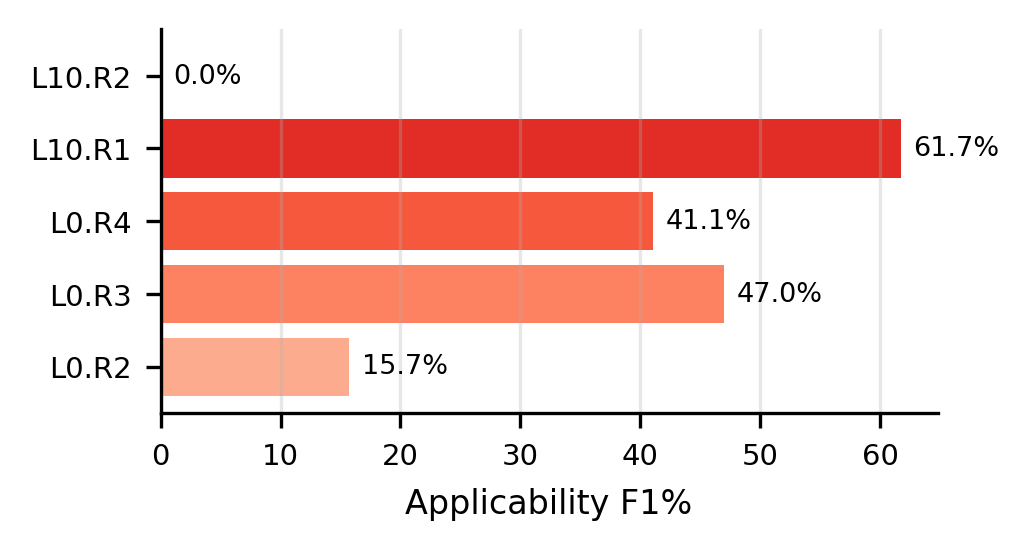
\includegraphics[width=\textwidth]{Figures/rule_breakdown_a.png}
\caption{Tier~0 (Safety)}
\end{subfigure}
\hfill
\begin{subfigure}[t]{0.48\textwidth}
\centering
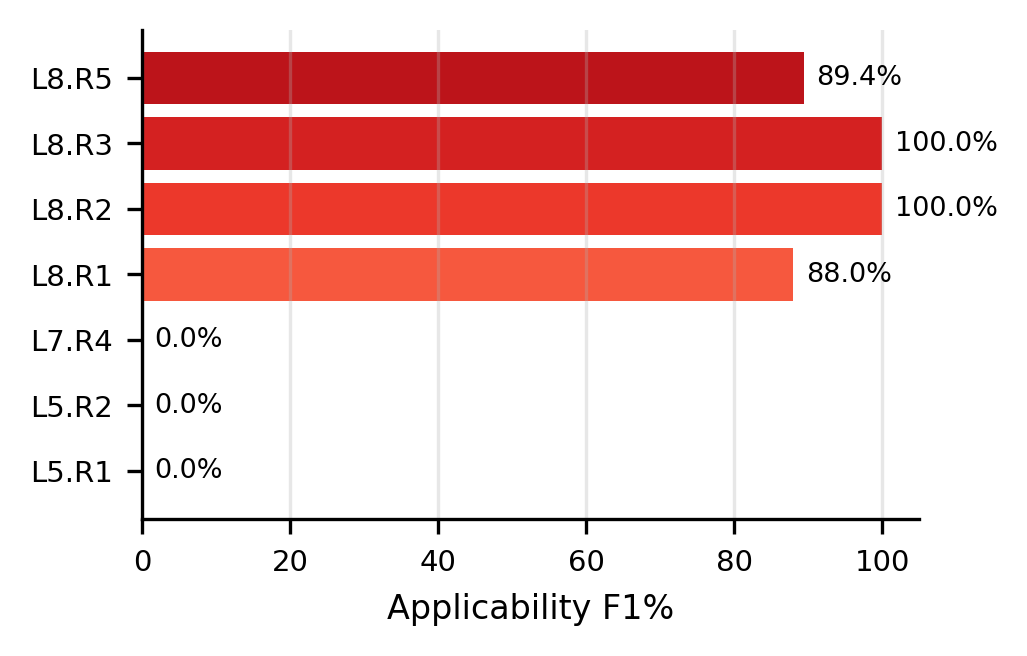
\includegraphics[width=\textwidth]{Figures/rule_breakdown_b.png}
\caption{Tier~1 (Legal)}
\end{subfigure}
\caption{Per-rule applicability F1 scores for RECTOR predictions (WOMD v1.3.0 \texttt{validation\_interactive}, diagnostic sample: 500~GT / 337~RECTOR scenarios), grouped by tier. Bar labels follow the Waymo evaluator's internal convention; the mapping to the paper's tier notation is given in Table~\ref{tab:rule_catalog}.}
\label{fig:rule_breakdown}
\end{figure*}

The observed support imbalance motivates the conservative applicability ablations in Section~\ref{Sec:Accuracy_SectionRule-Compliance_Behavior_and_Efficiency}.

%-------------------------------------------------------------------------------
\subsection{Waymo Rule Evaluation Framework}
\label{subsec:waymo_framework}
%-------------------------------------------------------------------------------

We use the Waymo Open Motion Dataset rule-evaluation framework as the authoritative auditor because it provides consistent rule semantics, oracle applicability labels, and stable regression targets. For each scenario we extract agent trajectories, map features, traffic-control state, and rule metadata into a shared context object; Protocol~A evaluates only the proxy subset with predicted applicability, whereas Protocol~B evaluates the full rule catalog with oracle applicability.

%-------------------------------------------------------------------------------
\subsection{Smooth Proxy Functions}
\label{subsec:proxy_functions}
%-------------------------------------------------------------------------------

The full evaluator is non-differentiable, so RECTOR uses smooth proxies for both optional rule-shaped training losses and stable selection-time ranking. The proxies replace hard predicates with hinge-like penalties, soft indicator gates, or differentiable event detectors.

\subsubsection{Proxy Coverage}

Of the 28~cataloged rules, \textbf{24 have smooth proxy implementations}
(86\% coverage).  All Tier~0 (Safety) rules are covered, ensuring that the highest-priority constraints contribute a training signal. Table~\ref{tab:training_eval_comparison} summarizes the training versus evaluation protocol.

\begin{table}[h]
\centering
\caption{Training vs.\ Evaluation Comparison}
\label{tab:training_eval_comparison}
\begin{tabular}{lcc}
\toprule
\textbf{Aspect} & \textbf{Training} & \textbf{Evaluation} \\
\midrule
Rules evaluated & 24 (proxied) & 28 (all) \\
Applicability source & Predicted ($\hat{a}_r$) & Oracle ($a_r^*$) \\
Map context & Partial & Full \\
Gradient flow & Yes & No \\
Speed & Fast ($\sim$1\,ms) & Moderate ($\sim$5\,ms) \\
\bottomrule
\end{tabular}
\vspace{2mm}
\footnotesize
\textit{Note:} Training uses smooth proxies for 24/28 rules to provide a
gradient signal.  Evaluation uses the full Waymo framework with complete map
context for all 28 rules.
\end{table}

The four unproxied rules fall into two categories: one requires multi-agent intent reasoning, and three depend on map annotations that are not reliably available in WOMD v1.3.0. They remain audit-only under Protocol~B.

\subsubsection{Normalization of Proxy Severities}

Proxy outputs have heterogeneous units, so each proxy produces a raw severity $V_r(\tau;s)\ge 0$ and a normalized severity $\bar{V}_r(\tau;s)\in[0,1]$:
\begin{equation}
\bar{V}_r(\tau;s)=\min\!\left(1,\,\frac{V_r(\tau;s)}{\alpha_r}\right),
\end{equation}
where $\alpha_r{>}0$ is the per-rule normalization constant introduced in Section~\ref{Sec:Problem_Formulation}. In the released implementation, the linear normalization is replaced by an exponential cost map:
\begin{equation}
c_r(v) = 1 - \exp\!\bigl(-\kappa_r \cdot \max(0, v)\bigr),
\label{eq:exponential_cost}
\end{equation}
where $\kappa_r > 0$ controls how quickly the cost saturates. This still satisfies the normalization contract required by Proposition~\ref{thm:scalarization}.

\begin{table}[t]
\centering
\caption{Per-Rule Proxy Parameters: Softness Constants and Violation Thresholds}
\label{tab:proxy_constants}
\scriptsize
\setlength{\tabcolsep}{2pt}
\resizebox{\columnwidth}{!}{%
\begin{tabular}{llccll}
\toprule
\textbf{Rule ID} & \textbf{Tier} & $\boldsymbol{\kappa_r}$ & \textbf{Threshold} & \textbf{Unit} & \textbf{Violation Semantics} \\
\midrule
\multicolumn{6}{l}{\textit{Tier 0: Safety}} \\
L0.R0 & Safety & 2.0 & 2.0 & m & Longitudinal gap $< d_{\min}$ to lead vehicle \\
L0.R1 & Safety & 2.0 & 0.5 & m & Lateral clearance $< d_{\text{lat}}$ to any agent \\
L0.R2 & Safety & 3.0 & 2.0 & m & Ego within crosswalk clearance zone \\
L0.R3 & Safety & 2.0 & 0.0 & m & OBB penetration depth (SAT) $> 0$ \\
L0.R4 & Safety & 2.0 & 1.0 & m & Distance to VRU $< d_{\text{VRU}}$ \\
\midrule
\multicolumn{6}{l}{\textit{Tier 1: Legal}} \\
L1.R0 & Legal & 3.0 & 2.0 & m & Crossing stop line under red signal \\
L1.R2 & Legal & 2.0 & --- & m/s & Speed $> v_{\text{limit}} + v_{\text{tol}}$ ($v_{\text{tol}}{=}$5\,mph) \\
L1.R3 & Legal & 3.0 & 2.0 & m & Crossing stop line under red signal \\
L1.R4 & Legal & 3.0 & 0.5 & m/s & Min speed in stop zone $> v_{\text{stop}}$ \\
L1.R5 & Legal & 3.0 & 5.0 & m & Ego within crosswalk yield radius \\
L1.R6 & Legal & 2.0 & 2.356 & rad & Heading deviation $>$ 135$^\circ$ from lane direction \\
\midrule
\multicolumn{6}{l}{\textit{Tier 2: Road}} \\
L2.R0 & Road & 2.0 & 1.0 & m & Signed distance outside drivable surface \\
L2.R1 & Road & 2.0 & 1.8 & m & Lateral offset $>$ half lane width $+$ margin \\
\midrule
\multicolumn{6}{l}{\textit{Tier 3: Comfort}} \\
L3.R0 & Comfort & 2.0 & 3.0 & m/s$^2$ & Longitudinal acceleration $> a_{\max}$ \\
L3.R1 & Comfort & 2.0 & 4.0 & m/s$^2$ & Braking deceleration $> a_{\text{brake}}$ \\
L3.R2 & Comfort & 2.0 & 0.5 & rad/s & Steering rate $> \omega_{\max}$ \\
L3.R3 & Comfort & 2.0 & 2.0 & m/s & Speed change $> \Delta v_{\max}$ \\
L3.R4 & Comfort & 2.0 & 2.0 & m/s$^3$ & Jerk $> j_{\max}$ \\
L3.R5 & Comfort & 2.0 & 4.0 & s & Left-turn TTC gap $< t_{\min}$ \\
L3.R9 & Comfort & 2.0 & 3.0 & s & Lane-change TTC $< t_{\min}$ \\
L3.R10 & Comfort & 2.0 & 2.0 & s & Following time $< t_{\text{follow}}$ \\
L3.R11 & Comfort & 2.0 & 3.0 & s & Intersection TTC $< t_{\min}$ \\
L3.R12 & Comfort & 2.0 & 3.0 & m & Pedestrian proximity $< d_{\text{VRU}}$ \\
L3.R13 & Comfort & 2.0 & 3.0 & m & Cyclist proximity $< d_{\text{VRU}}$ \\
\bottomrule
\end{tabular}%
}
\vspace{1mm}
\caption*{\footnotesize $\kappa_r$: softness parameter in the exponential cost function (Eq.~\ref{eq:exponential_cost}).  Higher $\kappa_r$ causes faster saturation to the maximum cost.  Signal-related proxies (L1.R0, L1.R3--R5, L0.R2) use $\kappa_r{=}3.0$; all others use $\kappa_r{=}2.0$.  Threshold: the physical limit above which the proxy begins to penalise; for rules where the threshold is inherent to the violation definition (e.g., speed limit), ``---'' indicates the threshold is scenario-dependent.  L1.R1 (priority), L3.R6--R8 (zone rules) are omitted as they lack proxy implementations.  Additional penalty scaling factors: yellow-light violations are scaled by 0.3$\times$, flashing-red by 0.5$\times$.}
\end{table}
%-------------------------------------------------------------------------------
\subsection{Proxy Implementation Details}
\label{subsec:proxy_details}
%-------------------------------------------------------------------------------

We report representative proxies, one per tier; the remaining proxies follow the same hinge-based or event-based pattern with parameters listed in Table~\ref{tab:proxy_constants}. All proxies are evaluated at 10\,Hz from decoded trajectories and derived kinematics.

\textbf{Safety (L0.R3 collision avoidance).}
\begin{equation}
V_{\text{L0.R3}}(\tau; s)=\sum_{t=1}^{T}\sum_{j\in\mathcal{A}_t}\min\!\left(p_{\text{long}}(t,j),\,p_{\text{lat}}(t,j)\right),
\end{equation}
where $p_{\text{long}}$ and $p_{\text{lat}}$ are SAT-style overlap depths along the vehicle axes.

\textbf{Legal (L1.R3 red-light stop).}
\begin{equation}
V_{\text{L1.R3}}(\tau; s)=\sum_{t=1}^{T} r(t)\,\sigma_\alpha\!\left(\mathrm{cross}(t)-\mathrm{cross}(t{-}1)\right),
\end{equation}
with $r(t)$ a soft red-signal indicator and $\mathrm{cross}(t)$ a differentiable stop-line crossing measure.

\textbf{Road (L2.R1 lane departure).}
\begin{equation}
V_{\text{L2.R1}}(\tau; s)=\sum_{t=1}^{T}\max\!\left(0,\,|d_t^{\text{lat}}|-\frac{w_{\text{lane}}}{2}-m\right),
\end{equation}
where $d_t^{\text{lat}}$ is signed lateral offset from the lane centerline.

\textbf{Comfort (L3.R4 jerk limiting).}
\begin{equation}
V_{\text{L3.R4}}(\tau; s)=\sum_{t=1}^{T-2}\max\!\left(0,\,|j_t|-j_{\max}\right).
\end{equation}

%-------------------------------------------------------------------------------
\subsection{Data Pipeline}
\label{subsec:data_pipeline}
%-------------------------------------------------------------------------------

The same rule-evaluation machinery is used during proxy-based training and full-catalog auditing.

Dataset statistics and splits are given in Section~\ref{Sec:Experiments}. The evaluation set spans dense intersections, freeway merges, lane changes, and other interaction-rich geometries, which is why the rule catalog must cover both high-priority safety events and lower-priority comfort behaviors.

Raw TFRecord scenarios are converted into ego-centric tensors by transforming coordinates to the ego frame, selecting nearby agents and relevant lanes, extracting finite-difference kinematics, and vectorizing map primitives such as lane polylines, stop lines, crosswalks, and drivable-surface polygons. Standard spatial and temporal augmentation is summarized in Table~\ref{tab:data_augmentation}.

\begin{table}[h]
\centering
\caption{Data Augmentation Strategies}
\label{tab:data_augmentation}
\begin{tabular}{llp{4cm}}
\toprule
\textbf{Augmentation} & \textbf{Parameters} & \textbf{Purpose} \\
\midrule
Rotation & $\pm 15^\circ$ & Orientation invariance \\
Translation & $\pm 2.0\,\mathrm{m}$ & Position invariance \\
Scaling & $0.95$--$1.05$ & Scale robustness \\
Agent dropout & 10\% prob. & Occlusion handling \\
Trajectory noise & $\mathcal{N}(0, 0.1^2)\,\mathrm{m}$ & Smoothness regularisation \\
Time reversal & 50\% prob. & Temporal symmetry \\
Mirror flip & 50\% prob. & Left-right symmetry \\
\bottomrule
\end{tabular}
\vspace{2mm}
\footnotesize
\textit{Note:} Augmentations are applied in the ego-centric frame.  Agent dropout simulates occlusions; trajectory noise regularises dynamics; mirror flips and rotations improve spatial invariance.  Rule-targeted augmentation generates synthetic samples with controlled violations to balance the proxy
supervision.
\end{table}

We additionally generate synthetic collision, speed, lane-departure, and red-light violations to improve proxy supervision on rare but high-impact events.
